\documentclass[11pt]{article}
\usepackage[T1]{fontenc}
\usepackage[utf8]{inputenc}
\usepackage[spanish,es-nodecimaldot,es-noshorthands]{babel}
\usepackage{lmodern,microtype,amsmath,graphicx}
\usepackage[a4paper,margin=20mm,headheight=15pt]{geometry}
\usepackage{array,booktabs,tabularx}
\usepackage{tikz}
\usetikzlibrary{positioning,arrows.meta}
\usepackage{xcolor,fancyhdr}
\definecolor{tinta}{HTML}{193045}
\definecolor{teal}{HTML}{116A61}
\definecolor{gris}{HTML}{4A5C6A}
\definecolor{suave}{HTML}{EAF4F3}
\usepackage[colorlinks=true,allcolors=teal,bookmarksnumbered=true]{hyperref}
\pagestyle{fancy}
\fancyhf{}
\fancyhead[L]{\small\color{gris} ROBÓTICA AVANZADA · UNITREE GO2}
\fancyhead[R]{\small\color{gris} PROYECTO FINAL · 2026-2}
\fancyfoot[R]{\small\color{gris}\thepage}
\renewcommand{\headrulewidth}{.3pt}
\setlength{\parindent}{0pt}
\setlength{\parskip}{.5em}
\setlength{\fboxsep}{8pt}
\renewcommand{\arraystretch}{1.18}
\newcolumntype{L}{>{\raggedright\arraybackslash}X}
\newcommand{\recuadro}[1]{\par\noindent\colorbox{suave}{\parbox{\dimexpr\linewidth-2\fboxsep}{#1}}\par}
\newcommand{\repo}{https://github.com/daca2022/go2-rl-deploy}

\hypersetup{pdftitle={Locomoción del Unitree Go2 con PPO y control de posición en MuJoCo}}
\renewcommand{\refname}{Referencias}
\begin{document}
\color{tinta}

{\color{teal}\small\bfseries PROYECTO FINAL · INFORME ACADÉMICO\par}
\vspace{.7em}
{\fontsize{31}{34}\selectfont\bfseries Locomoción del Unitree Go2\par}
\vspace{.35em}
{\Large PPO y control articular de posición en MuJoCo\par}
\vspace{.9em}
{\color{gris}Robótica avanzada · Ciclo 2026-2 · 18 de noviembre de 2026\par}

\section{Introducción}
Generar locomoción cuadrúpeda exige coordinar doce articulaciones, mantener el equilibrio durante los cambios de apoyo y seguir consignas de velocidad. Se implementó un controlador que combina una política entrenada con aprendizaje por refuerzo y realimentación proporcional-derivativa (PD). Se ensayó en MuJoCo \cite{todorov2012} con avance, retroceso, desplazamiento lateral y giro.

La pregunta experimental es si preparar un entrenamiento para incorporar dificultad progresiva mejora el seguimiento y la estabilidad frente a una referencia entrenada en plano nominal, al igualar el número de transiciones. Para responderla se contrastan dos entrenamientos A0/P0, E1 y E5, y se conserva una prueba preliminar independiente con una política recurrente A2/P0.

\recuadro{\textbf{Resumen.} En 138 episodios comunes, E1 aprobó 100 y E5 aprobó 98. Ambos completaron el mismo número de transiciones de aprendizaje. E1 conservó mayor margen en avance con masa y retardo. E5 aprobó más episodios en terreno rugoso y prolongó el retroceso en pendiente. La comparación describe dos corridas con una semilla de entrenamiento.}

\medskip
\begin{center}
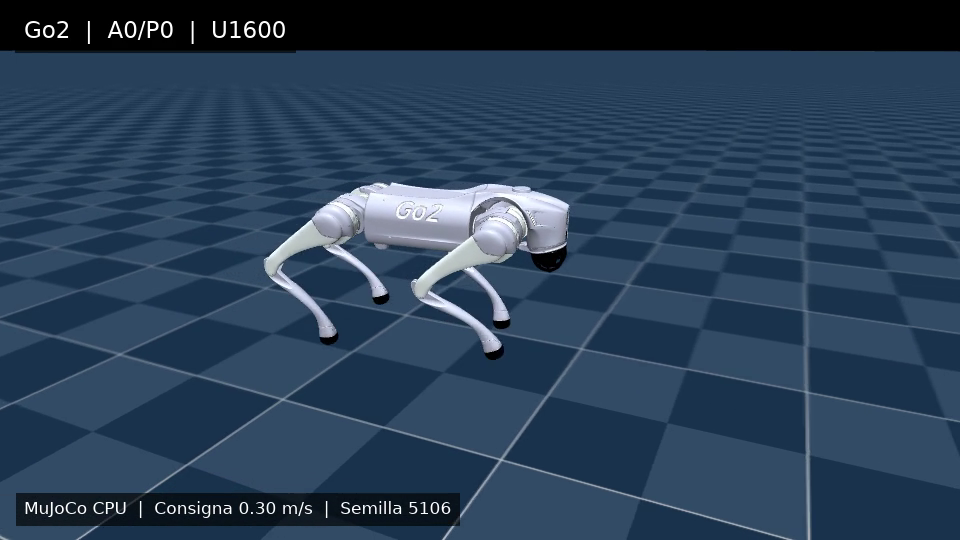
\includegraphics[width=.77\linewidth]{Fotograma-A0-U1600.png}

\footnotesize\textbf{Figura 1.} Fotograma del replay A0/P0 U1600 en MuJoCo CPU. El video muestra un episodio de desarrollo de avance de 20 s sin caída. Los resultados de E1 y E5 corresponden a U2000.
\end{center}

\href{https://drive.google.com/drive/folders/1S8uEebuWrVEXju7h-1b8J_P_9BeeqBDS}{Entrega pública y video en Drive}\quad
\href{\repo}{Código y política A2 en GitHub}

\newpage
\section{Metodología}
\subsection{Control y generación de movimiento}
La simulación de cuerpo rígido, juntas y contactos se ejecutó en MuJoCo. La integración física usa un paso de 5 ms y el actor se actualiza cada cuatro pasos, a 50 Hz. En A0, una red multicapa con capas ocultas 512, 256 y 128 recibe 47 valores. Estas entradas incluyen giroscopio, gravedad proyectada, consigna, posición y velocidad articulares, acción anterior y fase de marcha. A2 añade un estado recurrente con una GRU de 128 unidades \cite{cho2014}.

El actor produce 12 acciones adimensionales. Para la articulación \(j\), el control P0 calcula un objetivo de posición \(q_j^*\) y el actuador simulado aplica torque PD saturado:
\[
 q_j^* = q_{0,j}+0{,}25\,a_j,\qquad
 \tau_j = \operatorname{clip}_{[-\tau_{\max,j},\,\tau_{\max,j}]}
       \bigl(K_{p,j}(q_j^*-q_j)-K_{d,j}\dot q_j\bigr).
\]
Por pata, en el orden cadera, muslo y pantorrilla, se fijaron \(K_p=(20,20,40)\) N\,m/rad, \(K_d=(1,1,2)\) N\,m\,s/rad y límites \((23{,}5,23{,}5,45)\) N\,m. La realimentación PD regula las juntas. La política coordina los apoyos para seguir el movimiento pedido.

\begin{center}
\begin{tikzpicture}[
  nodo/.style={draw=teal,fill=suave,rounded corners=2pt,align=center,text width=3.05cm,minimum height=12mm,font=\small},
  flujo/.style={-{Stealth[length=1.8mm]},thick,draw=teal},
  node distance=5mm]
\node[nodo] (o) {Consigna y\\observación};
\node[nodo,right=of o] (a) {Actor\\A0 o A2};
\node[nodo,right=of a] (p) {Control P0\\posición y PD};
\node[nodo,right=of p] (m) {Go2 en MuJoCo\\juntas y contactos};
\draw[flujo] (o)--(a);
\draw[flujo] (a)--(p);
\draw[flujo] (p)--(m);
\draw[flujo] (m.south) -- ++(0,-.7) -| node[near start,below,font=\scriptsize]{realimentación de estado} (o.south);
\end{tikzpicture}

\footnotesize\textbf{Figura 2.} Lazo de control. El diagrama editable amplía el entrenamiento y la evaluación.
\end{center}

\subsection{Entrenamiento con PPO}
Proximal Policy Optimization (PPO) usa trayectorias recolectadas con la política vigente y limita el incentivo de hacer cambios grandes en las probabilidades de acción \cite{schulman2017}. Se ejecutaron 64 entornos con 24 pasos por actualización. La recompensa del proyecto combina seguimiento lineal y angular, patrón de trote y despeje del pie con regularización de postura, cambios de acción, deslizamiento y terminación. El trabajo de Rudin et al. \cite{rudin2022} sustenta la recolección paralela y el uso de currículos en locomoción. Hwangbo et al. \cite{hwangbo2019} muestran la importancia del modelo dinámico y de actuación para la transferencia física.

\newpage
\subsection{Diseño del contraste A0/P0}
E1 y E5 usan PPO, semilla de entrenamiento 7, cuatro consignas completas, 2.000 actualizaciones y \(2.000\times64\times24=3.072.000\) transiciones cada uno. Las consignas de referencia son avance \(0{,}30\) m/s, retroceso \(-0{,}20\) m/s, lateral \(0{,}20\) m/s y giro \(0{,}30\) rad/s.

\begin{tabularx}{\linewidth}{@{}p{.21\linewidth}LL@{}}
\toprule
 & \textbf{E1 · Referencia} & \textbf{E5 · Progresivo}\\
\midrule
Experiencia recolectada & Plano nominal durante todo el entrenamiento. & Plano durante todo el entrenamiento. La primera promoción se produjo al finalizar U2000.\\
Entorno & Reinicio y altura del pie nativos. & Ruta preparada para variar condiciones, reinicio físico propio y altura del pie sobre la superficie local.\\
Agenda & PPO continuo. & PPO por bloques. Las 125 pruebas internas usan pesos congelados.\\
Tiempo total & 2 h 12 min. & 6 h 20 min, con unas 4 h 01 min de revisiones internas.\\
\bottomrule
\end{tabularx}

El presupuesto de aprendizaje se expresa en transiciones. Las pruebas internas de E5 toman tiempo de cómputo y no alimentan las actualizaciones de PPO. Los multiplicadores declarados de recompensa coinciden. La implementación del término de despeje del pie y el entorno difieren, por lo que la equivalencia de multiplicadores no garantiza la misma señal de entrenamiento.

\subsection{Protocolo de evaluación}
Se usaron episodios de hasta 20 s en siete condiciones. Las cinco semillas de validación (1001 a 1005) se combinaron con cuatro consignas. Se emparejó por condición, consigna y semilla. Coincidieron la identidad de emparejamiento y las seis huellas de modelos compilados, mientras que las huellas completas de realización por corrida son distintas. El CSV conserva ambas huellas para auditar ese alcance. Los dos episodios ausentes de E1 se excluyeron de la comparación común y se conservan para E5.

El éxito requiere llegar al horizonte sin caída y cumplir el monitor de trote, que incluye patrón de apoyos y umbrales de seguimiento. El límite lineal es \(0{,}10\) m/s y el angular \(0{,}15\) rad/s. Se usa la raíz del error cuadrático medio (RMSE); para velocidad en el plano se computa
\[
 \mathrm{RMSE}_{xy}=\sqrt{\frac{1}{T}\int_0^T
                  \|\mathbf v_{xy}(t)-\mathbf v_{xy}^{*}(t)\|_2^2\,dt}.
\]
Se contabilizaron las caídas por separado y se retuvo el tiempo hasta el final del episodio. El test reservado se mantiene separado de los episodios descritos aquí.

\newpage
\section{Resultados}
\subsection{Robustez de E1 y E5 sobre 138 episodios comunes}
\begin{center}
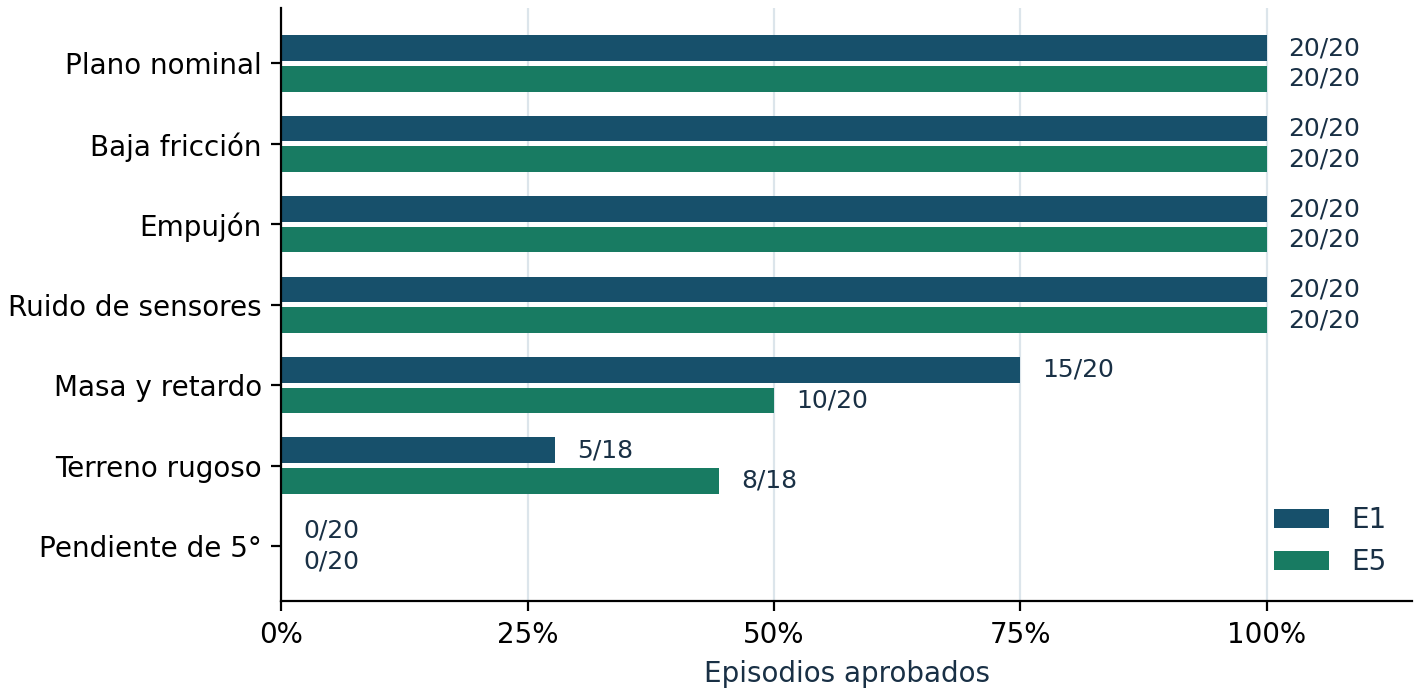
\includegraphics[width=\linewidth]{Resultados-por-escenario.png}

\footnotesize\textbf{Figura 3.} Aprobación por escenario. Se muestran los numeradores y denominadores del conjunto común.
\end{center}

\textbf{Resultado global.} E1 logró 100/138 y registró cinco caídas. E5 logró 98/138 y registró diez caídas. El registro completo de E5 contiene 99/140. Los dos episodios adicionales se ejecutaron en terreno rugoso: aprobó el giro y falló el lateral. Los dos entrenamientos lograron 20/20 por separado en plano, baja fricción, empujón y ruido.

\textbf{Masa y retardo.} E1 aprobó 15/20 y E5 aprobó 10/20, ambos sin caídas en esa condición. El lateral quedó en 0/5 para los dos. La diferencia de cinco aprobados salió del avance. Con masa y retardo el RMSE mediano de avance subió \(0{,}0309\) m/s en E1 y \(0{,}0289\) m/s en E5. E1 partía con menor error en plano y conservó margen frente al umbral. E5 cruzó \(0{,}10\) m/s.

\begin{center}
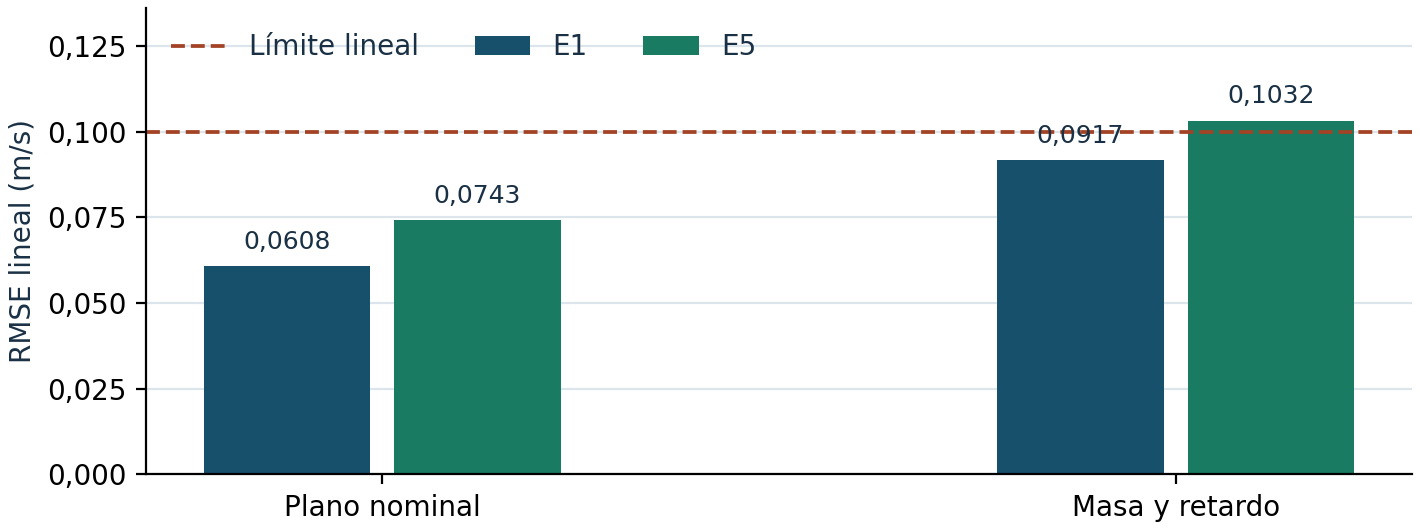
\includegraphics[width=.87\linewidth]{Error-de-avance.png}

\footnotesize\textbf{Figura 4.} RMSE lineal mediano de avance. Cada barra reúne cinco episodios. La línea indica el límite de aprobación lineal.
\end{center}

\newpage
\subsection{Pendiente y terreno rugoso}
En pendiente de \(5^\circ\) ambas políticas registraron 0/20 aprobados. En retroceso cayeron en los cinco casos, con medianas de 6,20 s para E1 y 14,90 s para E5. Al girar, E1 completó el horizonte sin caída en los cinco episodios y E5 cayó en los cinco, con mediana de 13,94 s. Esa diferencia explica las cinco caídas adicionales de E5. En terreno rugoso, E5 aprobó 8/18 frente a 5/18 de E1, con la mejora concentrada en retroceso.

\subsection{Qué explica la ventaja de la referencia}
Los dos completaron el mismo número de transiciones, y ambos practicaron en plano. En masa y retardo, el menor error de E1 en plano explica que el deterioro mediano observado dejara el avance de E1 bajo el umbral. Cotejar las muestras internas ubica el origen de trayectorias diferentes antes del primer control: la primera acción y recompensa coinciden, el segundo paso presenta pequeñas diferencias de dinámica, y hacia U20 ya se separan las trayectorias. La implementación del despeje, la geometría y el reinicio son factores que se pueden separar en una ablación. Los registros actuales permiten ubicar cuándo divergieron y qué métricas cambian.

Xie et al. \cite{xie2021} documentan casos de buena tolerancia de un cuadrúpedo entrenado sin aleatorización de dinámica. Engstrom et al. \cite{engstrom2020} muestran la sensibilidad de PPO a detalles de implementación. Henderson et al. \cite{henderson2018} sustentan la necesidad de variar semillas de entrenamiento antes de afirmar que una receta es superior. Estos trabajos orientan las hipótesis del proyecto.

\subsection{A2/P0 recurrente y demostración funcional}
En una revisión interna con el límite lineal común de \(0{,}10\) m/s, U2000 y U2800 aprobaron 20/20 en plano. El RMSE lateral fue \(0{,}09481\) y \(0{,}09322\) m/s respectivamente. En retroceso sobre \(+1^\circ\), U2000 cumplió el monitor en 5/5 y U2800 en 0/5, aunque ambos completaron 5/5 sin caída. Las repeticiones fueron deterministas. Se eligió U2000 para exportar el actor y probarlo por DDS local en MuJoCo, con cuatro ensayos de 20 s, 1.000 decisiones por consigna y cero caídas.

\begin{tabularx}{\linewidth}{@{}Lrr@{}}
\toprule
\textbf{Consigna en DDS} & \textbf{RMSE en plano (m/s)} & \textbf{RMSE de giro (rad/s)}\\
\midrule
Avance & 0,0620 & 0,0236\\
Retroceso & 0,0675 & 0,0241\\
Lateral & 0,0948 & 0,0189\\
Giro & 0,0176 & 0,0452\\
\bottomrule
\end{tabularx}

\medskip
Las métricas DDS verifican el recorrido de mensajes y la exportación del controlador en simulación. La validación reservada de A2 y la marcha con la política en el Go2 físico están pendientes en este corte.

\newpage
\section{Conclusiones}
Se implementó y demostró locomoción del Go2 en un simulador dinámico, con generación aprendida de objetivos articulares y seguimiento por control PD. El replay A0 evidencia el trote en plano. La prueba A2 recorre la exportación del actor y el intercambio de mensajes por DDS en MuJoCo para las cuatro consignas.

E1 mantiene la referencia para avance bajo masa y retardo y estabilidad al girar en pendiente. E5 ofrece una mejora puntual en terreno rugoso y más tiempo de estabilidad al retroceder en pendiente. Al igualar transiciones, el tiempo adicional de E5 corresponde principalmente a revisiones internas. La diferencia de dos aprobados y la falta de réplicas de entrenamiento dejan abierta la elección de una receta general.

El contraste causal propuesto parte del mismo checkpoint para dos ramas de igual presupuesto, conserva una en plano e incorpora pendiente leve efectiva en la otra. Se verificará el desempeño en plano y en pendiente en cortes emparejados. Para explicar la divergencia temprana desde cero se requiere otro contraste que aísle un cambio de entorno por vez y repita las semillas de entrenamiento. En una fase posterior, un maestro con estado privilegiado y un estudiante con observaciones disponibles podrían servir para investigar adaptación, como motiva la literatura de locomoción \cite{kumar2021}. La destilación y la comparación completa A0/A1/A2 con P0/T0 quedan fuera de los resultados demostrados en este informe.

\subsection*{Material reproducible}
El CSV documenta los 278 episodios registrados junto con la marca de pertenencia al conjunto común. Se incluyen las huellas SHA-256 de origen, el script de figuras, el diagrama editable y el video A0. El repositorio público contiene el actor A2, su modelo dinámico, el panel y la guía de ejecución. Los anexos distinguen episodios de desarrollo, validación, prueba de integración y aceptación del equipo físico.

\href{\repo}{Repositorio público y guía de MuJoCo}\quad
\href{https://drive.google.com/drive/folders/1S8uEebuWrVEXju7h-1b8J_P_9BeeqBDS}{Carpeta pública de material}


\newpage
\section*{Anexo de avance · 18 de noviembre de 2026}

\subsection*{Demostración lateral A2/P0}
El replay del GRU U2000 ejecutó 1.000 decisiones y 4.000 subpasos físicos en MuJoCo CPU. La demostración duró 20 s, con cero caídas según el criterio diagnóstico. Ante una consigna lateral de \(0{,}20\) m/s, la velocidad lateral media fue \(0{,}11021\) m/s y el RMSE planar fue \(0{,}09483\) m/s. El video y el CSV de telemetría permiten revisar tanto el desplazamiento como el margen de seguimiento.

\subsection*{Dos revisiones de desarrollo de la continuación}
Esta rama toma U2000 como punto de partida y programa cinco bloques hasta U4000. Se verificaron 50 episodios de las dos primeras revisiones. En el corte de publicación, el último registro de entrenamiento era U2940 y el recibo final seguía pendiente.

\begin{tabularx}{\linewidth}{@{}p{.14\linewidth}p{.18\linewidth}p{.20\linewidth}L@{}}
\toprule
\textbf{Corte} & \textbf{Aprobados en plano} & \textbf{Plano sin caída a 20 s} & \textbf{Reto propio del corte}\\
\midrule
U2400 & 20/20 & 20/20 & Retroceso en \(+1^\circ\). Cinco aprobados.\\
U2800 & 10/20 & 20/20 & Retroceso en \(+5^\circ\). Cinco sin caída y cero aprobados.\\
\bottomrule
\end{tabularx}

En U2800, avance y lateral nominales alcanzaron el horizonte con RMSE medio de \(0{,}13513\) y \(0{,}10729\) m/s. Ambos exceden el límite de \(0{,}10\) m/s. Los retos de pendiente tienen distintas inclinaciones. U2400 queda como candidato provisional hasta revisar los cinco bloques. Los 140 episodios reservados permanecen separados.

\subsection*{Preparación de la campaña}
Las seis combinaciones A0/A1/A2 con P0/T0 verificaron en CPU la construcción, PPO corto y la recarga de checkpoints. El catálogo de 2.800 actualizaciones conserva los 140 episodios emparejados por celda. La campaña de calidad y el cierre de las cuatro habilidades siguen pendientes. La prueba de reanudación DC en CPU reprodujo una actualización completa en otro proceso con igualdad de acciones, física y estado de entrenamiento. Quedan por verificar su uso en producción y su contabilidad acumulada de pared y disco.

\href{\repo/tree/main/docs/academico}{Presentación, videos, datos e índice de reproducibilidad}

\newpage
\begingroup\small
\bibliographystyle{unsrturl}
\bibliography{Referencias}
\endgroup
\end{document}
